\documentclass{trlnotes}
\usepackage{trmath}
\addcompatiblelayout{thesis}
\setlayout{thesis}
\usepackage{trthm}
\usepackage{trsym} 
\usepackage{trphys}
\usepackage{silence}
% \usepackage{tikz}
\WarningFilter{latex}{Reference}
\graphicspath{{../../}}

\usepackage[
backend=biber,
sorting=none,
natbib=true,
style=authoryear,
language=russian
]{biblatex}
\addbibresource{../../thesisrefs.bib}
\begin{document}

Большая часть дисковых галактик во Вселенной содержат бар --- яркую морфологическую особенность, выделяющуюся на 
фоне остальной галактики. По данным современных инфракрасных 
обзоров они наблюдаются в 60\%-70\% галактик до красного смещения $z\sim 1$ \citep{marinova2007}.
В этом факте нет ничего неожиданного~"--- большая часть часть звёздных дисков в $N$-body моделях неустойчива
относительно формирования бара, и необходимы специальные условия чтобы подавить его образование. В качестве такого
фактора может выступать массивное тёмного гало \underdev или подсистема, обеспечивающая высокую
центральную концентрацию, например сверхмассивная чёрная дыра \citep{shen2004} или компактный балдж
\citep{saha2018}.\note{Хотя, конечно, тут пишут что нельзя полностью уничтожить бар чёрной дырой, но нужны ли такие
детали во введении?}

% \begin{figure}[htpb]
%   \centering
%   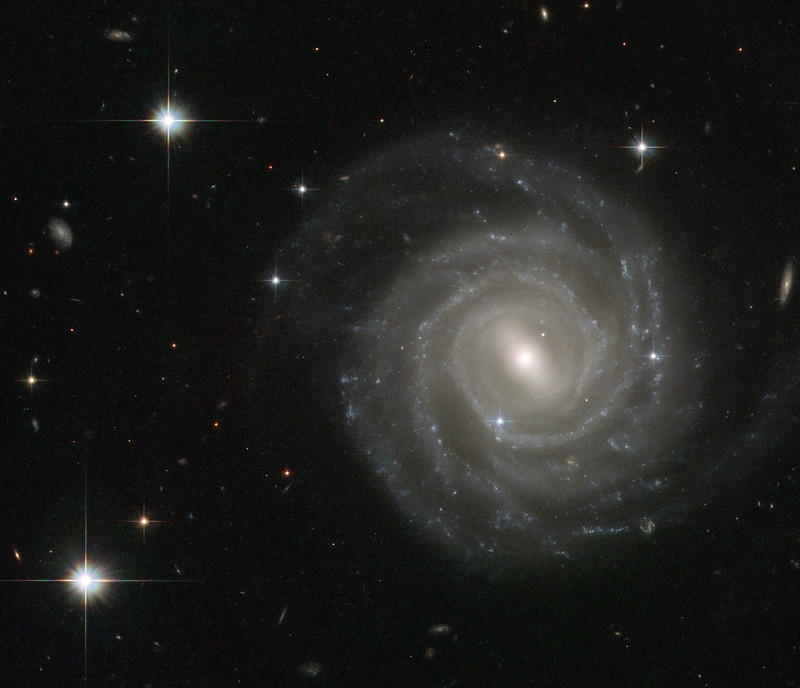
\includegraphics[width=0.8\linewidth]{img/intro/wp/ugc12158.jpg}
%   \caption{UGC 12158 --- галактика с выраженными спиральными рукавами и баром
%     \plholdev{а не барлинза ли тут, кстати}.
%     Пишут что она чем-то похожа на Млечный Путь, а снимок был снят чтобы запечатлеть
%     сверхновую SN 2004e.
%   Credit: ESA/Hubble \& NASA}%
%   \label{fig:frontpic}
% \end{figure}
%
% бессовестно скатано (не без неточностей) из обзора Атанасуллы в Secular evolution in disk galaxies
Как было показано в классических работах \citet{combes1981a} и \citet{raha1991} через непродолжительное время после
образования бара в модели, он <<выгибается>> из плоскости диска и на непродолжительное время теряет симметрию относительно неё. В
результате, галактика при взгляде с ребра приобретает ящикообразную или арахисообразную структуру, значительное
более утолщённую чем изначальный бар. Подобные особенности наблюдались в галактиках задолго до их обнаружения в
расчётах и, поскольку выступали за плоскость диска, были названы B/PS балджами. Например, в статье
\citet{burbidge1959} форма центрального региона галактики NGC 128 описана как необычная с наибольшей толщиной не в
центре диска, а в двух симметричных точках по обе стороны от центра\note{``...coming out of the nucleus itself like
a cross''!}, а в \citet{lutticke2000} из $\sim\!1350$ галактик видимых с ребра у $45\%$ были найдены B/PS балджи.
Многочисленные кинематические исследования установили прочную связь\note{это я так перевёл
established} между B/PS балджами и внутренней утолщённой в вертикальном направлении частью баров
\citep{kuijken1995,bureau1999,chung2004,bureau2006}. С точки зрения наблюдений,
наибольшую сложность представляет обнаружить бар в видимой с ребра галактике. В частности, в приведённых статьях
было показано, что наличие бара приводит к характерной форме распределения лучевой скорости с двумя высокими пиками и образует <<восьмёрку>> на диаграмме $R - v_{\text{loc}}$. 
Подобная корреляция проявляется и при изучении фотометрических характеристик, так в \citet{lutticke2000a} по форме
профилей в разреза вдоль большой оси и параллельно ей для 95\% галактик с B/PS структурами\note{из 60 рассмотренных...} было подтверждено наличие бара. 
К тому же, многие B/PS балджи вращаются цилиндрически, что в целом подтверждает их общую природу с баром. 
 
При взгляде на диск галактики <<плашмя>>, находясь вне её плоскости, установить наличие
или отсутствие в ней бара гораздо проще, например визуально или по увеличению эллиптичности изофот. Однако, при
этом необходима дополнительная информация, например, кинематические данные или металличность звёздного населения,
чтобы обнаружить B/PS балдж. В первом случае в качестве критерия чаще всего используется профиль параметра
$h^4$~"---  четвёртого члена в разложении в ряд Гаусса-Эрмита (\cite{vandermarel1993}) распределения лучевой
скорости вдоль большой оси бара. О существовании арахисообразной структуры при взгляде с ребра говорит наличие на
нём двух симметричных минимумов, обнаруженное в $N$-body моделях \citep{debattista2005,iannuzzi2015}) и наблюдениях \citep{mendez-abreu2008}.

% не менее бессовестно перевел кусок Laurikainen & Salo в книжке Galactic bulges
Однако, не менее интересно понять, к каким отличиям в морфологии бара <<плашмя>> приводит наличие B/PS балджа. 
Инструментом для подобного исследования может выступать анализ изофот, основная идея которого заключается в поиске
их отклонений  от эллипсов~"--- из $N$-body моделей вытекает, что для бара с B/PS балджем,
наблюдаемого на промежуточных углах наклона, изофоты должны иметь ящикообразную форму\note{не знаю на кого тут
сослаться}. Подобным образом с помощью NIR наблюдений обзора 2MASS  \citet{beaton2007} обнаружили B/PS структуру в Туманности Андромеды ($i = 77.5^\circ$). 
В \citet{erwin2013} были изучены 78 галактик на разных наклонениях с целью подобрать оптимальные параметры для
одновременного обнаружения бара и B/PS балджа. При этом, в этой работе после экстраполяции по выборке
подходящих галактик, авторы приходят к выводу, что 2/3 баров должны проявляться с ребра как B/PS балджи, что в
целом согласуется с выводами \citet{lutticke2000a}, но не очень надёжно в силу небольшого размера выборки.

Для галактик, наблюдаемых под небольшими углами наклона, возможна и отличная от ящикообразной морфология бара.
Довольно часто наблюдается линзовидные структуры, погруженные в бар в его центральной части. Подобная особенность
была впервые широко освещена в работе \citet{laurikainen2011} и была названа авторами \emph{барлинзой}.
Авторы статьи провели детальную классификацию $\sim\!200$ дисковых галактик ранних типов по наблюдениям в
инфракрасном диапазоне, добавив условное обозначение для барлинз (bl) в ранее описанные в литературе типы
\citep{devaucouleurs1959,buta2010}). От центральных линз (nuclear lens) и обычных линз они отличаются
размерами~"--- около половины длина бара, а от классических балджей~"--- профилем плотности и кинематическими
характеристиками. 

Таким образом, бары по их морфологии плашмя можно разделить на как минимум две выделяющиеся группы~"--- бары с
барлинзами и арахисообразные бары. Однако, статистические исследования числа баров разных типов представлены только в
нескольких работах, и пока нет общепризнанного взгляда на этот вопрос. Например, в анализе приведённом в
\citet{li2017a}, на небольших углах наклона ($0^\circ$ -- $40^\circ$) авторы нашли всего $3\%$ процента баров с
арахисообразной морфологией и $27\%$ барлинз от общего числа галактик, а на значительных углах наклона ($40^\circ$
-- $70^\circ$) эти доли составили $13\%$ и $12\%$ соответственно. При этом, доля галактик с баром в обоих
диапазонах отличается незначительно~"--- $74\%$ и $68\%$, так же как и доля галактик, бары в которых имеют
эллиптические изофоты (unbuckled в терминологии авторов). 

Природа барлинз и корреляция между числом баров разных типов на разных наклонениях не могли не вызывать интереса
исследователей в этой области. В статье \citet{athanassoula2013a} для моделей с учетом газа и физических процессов 
в нём (звездообразование, высвечивание и т.п) получилась вполне похожая на барлинзу морфология (например, ~Fig.~4 
оттуда), а в \citet{athanassoula2015} на основе сопоставимих размеров барлинз и B/PS балджей при фотометрической 
декомпозиции $N$-body моделей с учетом газодинамики делается вывод, что это проявления одной и той же структуры, 
видимой под разными углами наклона. В \cite{salo2017} авторы приходят к похожим выводам, анализируя, 
однако, бесстолкновительные симуляции с классическим балджем, заданным в качестве начального условия, а не 
образующегося в результате звездообразования в натекающем на центр галактики газе. 

Связь наблюдаемой морфологии бара с параметрами подстилающей галактики часто становится предметом исследований, 
анализующих $N$-body модели. Так, например в \citet{athanassoula2002} было рассмотрено три модели: с массивным гало 
($M_h/M_d = 1.5$), с массивным диском ($M_h/M_d = 0.75$) и с массивным диском и массивным классическим балджем 
($M_h/M_d = 0.75$, $M_b/M_d = 0.6$). При этом, в первом случае образовался выраженный бар, во втором случае~"--- 
скорее овалообразное искажение изофот, а в третьем~"--- что-то среднее. В уже упомянутой ранее 
статье \cite{salo2017} авторы отмечают, что крутая кривая вращения, связанная с наличием компактого классического 
балджа приводит к образованию бара с барлинзой, а более пологая при отсутствии балджа~"--- к арахисообразному 
бару. Важно отметить, что в последнем случае X-образные особенности проявляются даже при нулевом угле наклона.  
\citet{smirnov2018} подтвердили этот вывод и отметили, что варьирование других параметров модели, таких как 
параметр Тумре ($Q$) или начальная толщина диска ($Z_d$) могут приводить к возникновению барлинз в 
бесстолкновительных моделях даже при отсутствии балджа. Однако, их довольно сложно получить из наблюдательных 
данных, в отличие от массы и радиуса балджа, которые определяется при аккуратной фотометрической декомпозиции 
изображения галактики; например в \citet{laurikainen2014}) для приведённой выборки доля массы балджа составила
$0.1$, вместо $0.35$, получающейся при неучете барлизны. Важно отметить, что и в наблюдениях
\citep{laurikainen2017}, и в моделях \citep{salo2017} возникает промежуточная ситуация~"--- на изображениях с
барлинзами после применения нерезкого маскирования обнаруживаются X-образные детали (Fig~A.4, IC 1067 в первой
статье), причём даже в депроецированных изображениях. Этот факт явно свидетельствуют о динамической природе
морфологических различий. 

Анализ вертикальной структуры $N$-body моделей многокомпонентных галактик показывает связь параметров родительской
галактики с геометрическими параметрами B/PS структуры \citep{smirnov2018}, а не только с морфологией бара
<<плашмя>>. Подобная взаимосвязь основана на разнице в орбитальном составе B/PS балджей, образовавшихся в разных
потенциалах \citep{parul2020}. Вопрос об орбитах, поддерживающих трёхмерный бар, достаточно подробно освещён в
литературе (например в обзоре \cite{athanassoula2016}), однако, поскольку барлинзы были обнаружены относительно
недавно, их природа ещё во многом остаётся неизвестной. 


Цель данной работы~"--- детальное изучение разницы в орбитальном составе разных по морфологии баров, возникающих
в самосогласованных $N$-body моделях дисковых галактик. При этом интересовать нас будут именно различия
возникающие при наблюдении плашмя, а вертикальная структура практически не рассматривается. 
\begin{enumerate}
  \item В главе~\ref{chap:model} описаны параметры $N$-body моделей, приводящие к образованию бара с барлинзой и
    арахисообразного бара и используемая методика проведения $N$-body моделирования,
  \item Глава~\ref{chap:method} посвящена описанию основного метода, используемого в работе~"--- анализа
    доминирующих частот,
  \item Большая часть главы~\ref{chap:split} состоит в описании процедуры выделения орбитальных семейств~"---
    близких по морфологии групп орбит, и в сравнении населённости разных семейств для разных моделей, 
  \item И, наконец, в главе~\ref{chap:orb} приведены основные орбиты для каждого из разобранных семейств.
\end{enumerate}

\end{document}
% vim:wrapmargin=3
